\chapter{Modélisation du comportement des usagers}

La démarche de modélisation est une approche scientifique qui a pour but de produire de la connaissance sur des phénomènes naturels ou artificiels. Cette démarche est utilisée pour comprendre, prédire voire contrôler des phénomènes qu'ils soient déjà existants ou encore au stade de la conception. Le principe est de créer une simplification numérique du phénomène étudié. Les modèles sont donc souvent indispensables, mais ils sont également toujours faux. Les bons modèles sont des approximations qui apportent une plus-value pour la prévision de phénomènes.

Cette thèse s'intéresse à la modélisation du comportement des occupants pour la prédiction de la demande d'énergie. Pour cela, il est nécessaire de s'intéresser à l'interaction entre les occupants et leur environnement. Ces interactions sont de deux natures: la première concerne les gains dus aux apports métaboliques et les divers apports internes de chaleur; la seconde concerne l'utilisation des systèmes de l'environnement (fenêtres, volets, lumières, air conditionnée, etc.) qui sont régulés par les occupants et leurs besoins.

Réussir à modéliser les actions et comportements des usagers d'une manière cohérente et généralisée est important pour offrir aux industriels des méthodes et des logiciels adaptés à leur mission de conception de bâtiment. Ce chapitre présente alors les types de modélisation du comportement des occupants recensés dans la littérature et les plateformes numériques pouvant réaliser ces modélisations. 

\section{Familles de modèles}

Il existe deux grands types d'approche de modélisation, les approches descendantes (dites \textit{top-down} en anglais) et les approches ascendante (dites \textit{bottom-up} en anglais). Les modèles de demande d'énergie descendants comme celui qu'a développé Kelly et al. \cite{Kelly-13} utilise une analyse de régression d'une grande population pour déterminer l'influence des facteurs individuels. Alors que les modèles ascendants étudient en détails chaque composant pour les combiner et générer un résultat d'ensemble. C'est ce deuxième type d'approche qui est traité dans la suite de ce chapitre.

Au sein de ce type d'approche, nous avons réalisé une étude bibliographique qui nous a permis de distinguer six familles de modélisation du comportement des usagers à des fins énergétiques dans le contexte du bâtiment. Cette large revue des modèles existants est indispensable pour en comprendre les possibilités, forces et faiblesses de chacun afin de répondre aux objectifs initiaux. Les modèles dits: psychologiques, basés sur des valeurs moyennes, déterministes, probabilistes, utilisant les systèmes multi-agents et "action-based" sont présentés dans ce qui suit.

\subsection{Modèles psychologiques}

Les modèles psychologiques du comportement des occupants peuvent être distingués en deux groupes, ceux considérant le comportement individuellement et ceux en lien avec l'utilisation de l'énergie dans les bâtiments.

En effet, certains modèles psychologiques fonctionnent en utilisant comme indicateurs les besoins fondamentaux des êtres humains. Ces derniers se limitent d'une part aux besoins physiologiques des êtres humains: faim, soif, sexualité, respiration, sommeil, élimination selon la pyramide établie par le psychologue Maslow \cite{Maslow-56}. D'autre part à la notion de confort physiologique qui considère les aspects hygrothermiques, acoustiques, visuels et olfactifs. Dans un cadre de modélisation du comportement des usagers à des fins énergétiques, il va de soi que l'intégralité de ces besoins et types de confort ne sont pas pris en compte. 
Une fois les définitions des paramètres d'influences sélectionnés, l'objectif est de prédire les pratiques \footnote{En langue française on utilise comme synonyme "pratique" et "comportement" alors que la langue anglaise fait une distinction sémantique. "Behavior" désigne un geste observable et quantifiable, alors que "practice" renvoie à l'activité et permet d'insister sur son contexte de réalisation comme sur le sens que les individus lui attribuent} des usagers en fonction de la physiologie de la population et des normes sociales. En 1991, le psychologue social, Ajzen \cite{Ajzen-91}, a mis au point une théorie du comportement planifié de ce type, qui s'est révélée comme étant à l'origine de nombreux sous-modèles psychologiques. On y retrouve ces sous-modèles sous forme de boucles, généralement considérant connaissance, désir, capacité, attitude et finalement action. Ce terme de boucle est utilisé dans le sens où le modèle se présente comme un enchainement d'étapes qui sont répétées à chaque pas de temps de la simulation, comme un algorithme.

On a vu que certains modèles psychologiques sont uniquement basés sur la physiologie des occupants, alors que ce paragraphe consacré au deuxième type de modèles psychologiques, intègre la dimension économique. On retrouve une application dans le secteur résidentiel avec Van Raaij et al. \cite{VanRaaij-83} qui prennent soin de considérer le ménage lui-même, c'est à dire son niveau socio-démographique, son style de vie, le prix de l'énergie ou encore sa responsabilité devant l'énergie. En comparaison, aux modèles uniquement basés sur la physiologie, ces modèles se revendiquent comme plus complets car ils considèrent en outre la technologie, l'économie, la démographie, les institutions, la culture. Néanmoins, le principe de boucle n'est pas modifié et l'indicateur principal reste le bien être des occupants. Ici l'approche est plus transversale car elle n'est pas centrée uniquement sur la physiologie de l'occupant et son bien être mais considère également des paramètres qui influent effectivement sur le comportement.

\subsection{Valeurs moyennes}

Les modèles fondés sur des valeurs moyennes sont généralement considérés comme élémentaires par la communauté scientifique car leur flexibilité est très réduite. En effet, pour les différentes entrées du modèle on a des valeurs uniques. C'est donc sur ce principe que se base ce type de modélisation, si l'on cherche à étudier la sortie $y$ d'un phénomène, les entrées $x_1$, $x_2$, $...$ et $x_n$ sont des valeurs statiques, constantes au cours de la simulation. A titre d'exemple, Morel et Gnansounou de l'Ecole Polytechnique de Lausanne \cite{Morel-09} considèrent les gains internes des bâtiments résidentiels égaux à 5$W/m^{2}$. Ici la valeur importe peu, elle est d'ailleurs peut être proche de la réalité, mais sa limite réside dans l'impossibilité de la détailler selon des paramètres d'influence: type de pièce, nombre d'occupant, date et heure, etc. Cet exemple parmi tant d'autres permet de dire qu'un modèle basé sur des valeurs moyennes utilise des données totales comme paramètres d'entrée. Ces types de modèles fonctionnent alors sur l'implémentation de valeurs uniques dans l'algorithme de simulation, par conséquent, il en résulte automatiquement des valeurs également uniques pour chaque sortie.

L'application des modèles basés sur les valeurs moyennes est la plus appropriée pour estimer des consommations énergétiques d'un échantillon large de bâtiments. Comme nous le verrons dans les prochains paragraphes et alors qu'elle est également envisageable pour des bâtiments individuels, des modèles stochastiques ou à base d'agents produiront des résultats moins bruts, plus proches des pratiques possibles et seront donc plus appropriés à un niveau de modélisation supérieur.

\subsection{Modèles déterministes}

Les modèles déterministes, également appelés \textit{rule-based} par les anglophones, ont pour habitude d'être assimilés aux modèles des valeurs moyennes, dans le sens où leurs données d'entrée sont discutables car souvent basées sur des simplifications. Ces suppositions sont le fruit d'études sociologiques quantitatives trop peu nombreuses pour avoir une base de données suffisamment importante et fiable. Certaines données sont disparates et fiables mais tout de même à exploiter avec précaution, tant les paramètres d'influence sont nombreux.

Dans leur modèle, Glicksman et Taub \cite{Glicksman-97} cherchent à identifier les paramètres qui ont la plus grande influence sur l'efficacité énergétique. Dans cet article, la modélisation du comportement des habitants face au chauffage, à la ventilation et à l'air conditionné est faite de manière déterministe. Ce type de modèle simplifié et limité par son dynamisme est également utilisé dans l'outil de simulation thermique dynamique développé par Izuba, Pleiades+Comfie. Dans celui-ci, son cœur de calcul est pour l'utilisateur une boite noire, qui est seulement maître des données d'entrée. Après avoir renseigné le logiciel sur les éléments géométriques, environnementaux et les différents systèmes du bâtiment, le modélisateur doit définir de multiples scénarii d'utilisation. Pour chaque zone thermique, il doit déterminer: les consignes de température, les scénarii d'occupation, les puissances dissipées, les jeux d'occultation, les niveaux d'éclairement ou encore les besoins en eau chaude sanitaire. Cette détermination est réalisée heure par heure au travers de scénarii hebdomadaires répétitifs totalement décorrélés de la notion de confort. Or, on comprend la limite de considérer les comportements des usagers comme entièrement prévisibles et répétables.

\subsection{Modèles probabilistes}

Les processus probabilistes, également appelés stochastiques, utilisent des paramètres et équations qui évaluent les probabilités d'une action ou d'un changement d'état du système. Contrairement aux modèles basés sur des moyennes ou aux modèles déterministes, les modèles probabilistes se basent davantage sur des études statistiques qui proposent des profils. Les méthodes d'échantillonnage de distributions d'événements sont nombreuses. On retrouve fréquemment des méthodes de la transformée inverse, tel que dans le travail de Vorger sur l'influence des occupants sur la performance énergétique par le biais d'une modélisation stochastique globale \cite{Vorger-14} ou des méthodes de Monte-Carlo par chaînes de Markov, comme Tijani l'a fait pour le développement d'un modèle purement statistique \cite{Tijani-14} afin de le comparer aux systèmes multi-agents qui sont eux présentés dans la Section \ref{Systèmes Multi-Agents}. Dans le cadre de la modélisation du comportement, l'approche probabiliste permet de considérer les aléas comportementaux des humains. Cette approche demande de posséder une base de données suffisante pour connaitre les habitudes des occupants, d'où l'intérêt de campagnes de mesures et de questionnaires. Ces informations sur les habitudes des occupants concernent les tâches qui sont réalisées, leurs durées et leurs enchaînements. Les chaines de Markov sont alors le système mathématique qui correspond le mieux à ce besoin. En effet, les processus de Markov sont "sans mémoire" et permettent des transitions d'états pour des durées plus ou moins longues. Ils permettent ainsi de réaliser aléatoirement des changements d'états (positions, actions, activités, etc.) des occupants du modèle en intégrant préalablement les études statistiques. Concrètement, les chaines de Markov de premier degré fonctionnent de la manière suivante:
\begin{enumerate}
\renewcommand{\arraystretch}{0}
\item Étude des données temporelles d'activité, les probabilités cumulées de transition sont calculées
\item La matrice de probabilité de transition est calculée
\item Un nombre aléatoire compris entre 0 et 1 est généré
\item Le nouvel état est déterminé, en fonction de l'état précédent, du nombre aléatoire généré et des probabilités cumulées de transition
\end{enumerate}
Un modèle probabiliste avancé est développé dans le volume II: "Occupant behavior and modeling" de l'Annexe 53: Total energy use in buildings" \cite{Annex-53-1}, celui-ci présente une étude statistique préalable sur les consommations énergétiques, détermine la typologie du bâtiment et détermine les informations sur les occupants afin d'en sortir les localisations et activités de chaque occupant pour un pas de temps de 5 minutes. On notera tout de même que les sorties de ce modèle se limitent ici à la localisation et aux activités des occupants, alors qu'on peut imaginer que la finalité d'un tel modèle sera d'estimer les besoins énergétiques. Les modèles probabilistes et les méthodes de type aléatoire permettent de générer des événements ou échantillons extrêmes, tout en ayant conscience de la pondération des  résultats. En effet, c'est le principe de la Gaussienne, il est plus probable de générer un événement dans la moyenne qu'un événement extrême. En revanche, sur de nombreuses simulations les chaînes de Markov ressemblent à des modèles basés sur des valeurs moyennes, car les moyennes des événements aléatoires vont tendre vers les états les plus fréquents trouvés lors de l'étude statistique \cite{Annex-53-1}.

Pour synthétiser ce qu'est la modélisation stochastique on dit souvent qu'elle égale à une modélisation déterministe associée à une part d'aléatoire.

\subsection{"Action-based" modèles}

Les modèles axés sur les actions des occupants sont développés suivant deux volets: l'occupation des zones et les activités de leurs occupants. Dans ce type de modèle l'occupation est déterminée par la localisation des occupants qui est le résultat des mouvements d'une zone du bâtiment à l'autre. Tout comme pour les modèles probabilistes, ces déplacements d'une zone à l'autre sont généralement générés simplement par les méthodes des chaines de Markov et transitions d'états. Les activités des occupants sont générées aléatoirement et concernent les ouvertures de fenêtres, la gestion des lumières, de l'air conditionné ou encore de l'usage des appareils électroménagers. Ces modèles dits d'actions associent donc les comportements des usagers à des déplacements et à des actions concrètes sur les systèmes du bâtiment.

Comme pour les modèles stochastiques, la typologie des bâtiments, le nombre et les types d'occupants par zone sont renseignés au modèle pour le volet des déplacements des occupants. Cependant, la plus-value réside dans l'ajout d'informations supplémentaires concernant les horaires et durées des séjours et activités dans les zones étudiées \cite{Annex-53-1}. Cette modélisation des déplacements au sein du bâtiment, fixe ou suit l'évolution des systèmes à chaque pas de temps qu'ils soient booléens, discontinus ou continus. Pour les définitions des événements on note généralement six attributs à renseigner au modèle, les temps de début et fin, la localisation, les participants, les indicateurs statistiques et les priorités en cas de conflit. 

Comparés aux modèles déterministes où les actions sont prédéfinies et inchangeables, ces types de modèles considèrent le caractère aléatoire par une occupation inégale et asynchrone dans l'espace et le temps. On a une combinaison entre les modèles déterministes et probabilistes. La plus-value de ce modèle réside dans la personnalisation des occupants, même extrêmes, aussi bien dans leur génération que dans leurs comportements concrets devant les systèmes consommateurs d'énergie. Cependant, les modèles d'actions sont de type réactifs et ne prennent pas en compte les interactions entre les occupants du modèle.

\subsection{Systèmes Multi-Agents (SMA)}
\label{Systèmes Multi-Agents}

Les Systèmes Multi-Agents permettent d'établir des règles de comportement des usagers à travers de l'utilisation d'agents autonomes dont leur comportement est automatiquement calculé sans suivre des profils préétablis. Les modèles à base d'agents considèrent les occupants comme des entités individuelles capables de prendre des décisions selon leurs règles et expériences en étant interactif entre eux et avec leur environnement.

En réalité cette définition complexe est finalement assez souple et plusieurs niveaux d'agents sont généralement perçues. Ferber \cite{Ferber-95} classe les SMA en deux grandes catégories; la première est celle où les agents sont réactifs et reposent sur des actions prédéfinies et déclenchées automatiquement, tels des stimulus. Ces agents réactifs perçoivent leur environnement et agissent sur celui-ci en choisissant parmi des comportements prédéfinis, celui qui est les plus adapté à la situation. La deuxième catégorie de SMA est celle fonctionnant sur des agents cognitifs. Dans cette catégorie les agents possèdent des capacités de raisonnement et de mémorisation. Les agents les plus évolués peuvent même développer de nouvelles connaissances ou des organisations selon des paramètres sociaux, psychologiques et biologiques mais également en fonction des interactions avec les autres agents.

Dans le cadre de la modélisation des occupants dans le contexte du bâtiment et de la maitrise de l'énergie, Davidsson et Boman \cite{Davidsson-05} présentent un modèle multi-agents considérant lumière et chauffage. L'énumération suivante présente les relations simplifiées entre les agents et les conditions intérieures:
\begin{enumerate}
\renewcommand{\arraystretch}{0}
\item Quand aucun agent est dans la pièce, les conditions par défaut sont maintenues
\item Quand un agent entre dans la pièce, il adapte la température et allume les lumières selon ses préférences
\item Quand plusieurs agents sont dans la pièce, les conditions sont fixées en fonction des préférences des agents présents par délibération
\end{enumerate}
Davidsson et Boman \cite{Davidsson-05} utilisent bien des SMA, car les occupants sont assimilés à des agents autonomes aux propriétés individuelles qui leurs sont propres et qui plus est avec des interactions entre eux. Ces agents ne sont en revanche pas cognitifs puisqu'ils n'ont pas de capacité d'apprentissage et de mémorisation, c'est à dire qu'ils sont davantage pulsionnels qu'intentionnels.

Kashif \cite{Kashif-11} a quand à elle développé sous BRAHMS \footnote{BRAHMS est un logiciel développé par la NASA, permettant la simulation et l'analyse séquencée du comportement des agents lors de chaque processus de décision} des agents cognitifs ayant une perception de leur environnement et une capacité de délibération pour le contrôle et la gestion de l'énergie. Dans ce projet les mécanismes de réaction aux évènements prennent en compte une explicitation des buts, des mécanismes de planification et peuvent résoudre des problèmes qualifiés de complexes. Cette approche choisie par Kashif considérant les croyances, les désires, les contraintes, les perception et les états physiques mobilise une partie de la branche de l'intelligence artificielle en laissant apercevoir un potentiel jugé fort. Or à l'heure actuelle cette approche très fine ne permet pas d'avoir des résultats d'ensemble exploitables notamment en termes de consommations énergétiques. Tijani \cite{Tijani-14}, dans la continuité du travail de Kashif \cite{Kashif-11}, dans son article sur l'approche multi-agents du comportement des occupants avertit et confirme que malgré un fort potentiel des SMA, la complexité de BRAHMS rend l'application à l'énergétique des bâtiments et à la qualité de l'air intérieur difficile.

En plus des niveaux de détails des modèles qui dépendent des objectifs des projets, les disciplines insistent sur différents aspects du processus de décision humain:
\begin{itemize}
\renewcommand{\arraystretch}{0}
\item En psychologie, les agents sont créés autours de facteurs internes tels les croyances et désires. Soit les agents réagissent selon les théories d'actions normalisées de Schwartz \cite{Schwartz-77} ou soit selon les théories de comportement planifié d'Ajzen \cite{Ajzen-91}.
\item En économie, les agents sont créés autours de facteurs externes tels des indices du marché et autres aspects financiers. Ce sont ces paramètres rationnels économiques qui vont guider les décisions des agents.
\item En informatique, les agents sont créés à partir des connaissances de l'intelligence artificielle et propose des capacités évoluées d'autonomie. Savall \cite{Savall-03} au travers de son modèle d'organisation YAMAM montre comment la cognitivité est recherchée notamment par la possibilité de modifier des règles de comportement des agents en cours de simulation.
\end{itemize}
Ainsi, plusieurs sciences utilisent les Systèmes Multi-Agents à des fins diverses et aux niveaux de complexité et cognitivité hétéroclites. Les conditions communes minimales pour appeler les agents comme tels selon trois précurseurs des SMA: Erceau \cite{Erceau-93}, Ferber \cite{Ferber-95} et Maes \cite{Maes-95} sont de percevoir l'environnement, de décider selon des perceptions, puis d'agir sur l'environnement. 

\subsection{L'approche hybride socio-stochastique}

1- Utilisation des modèles stochastiques utilisés couramment lors de la modélisation des comportements des occupants.
- Méthode de la transformée inverse (Eric Vorger p37)
- Modèle linéaire multiple
- Chaines de Markov à temps discret 
- Analyse 

2- Intégration des phénomènes sociologiques en sortie des modèles stochastiques:
- Effet rebond
- Dynamique de groupe 
(- Contournement technologique) G. Brisepierre

\subsection{Synthèse}


%%%%%%%%%%%%%%%%%%
% Fit-to-purpose %
%%%% Gaetani %%%%%
%%%%%%%%%%%%%%%%%%
% Methodology:
% 1. What are the existing models/simulation frameworks for OB?
% 2. Which combination of factors influence the impact of OB on the predicted building energy performance?
% 3. What is the most fit-for-purpose OB modeling complexity level for a specific case 

Le choix du modèle dépend fortement des objectifs de la simulation mais aussi des logiciels choisis ou disponibles. On note que le développement d'un modèle se réalise souvent en couplant plusieurs modèles de base. Dans le tableau \ref{synthese modeles}, sont regroupés les six modèles présentés dans ce chapitre, leurs données d'entrée, leur développement, une référence et enfin les limites générales du modèle considéré. 

\begin{landscape}
\begin{table}
\centering
\begin{tabular}{|p{4.5cm}||p{4.5cm}|p{4.5cm}|p{4.5cm}|p{4.5cm}|p{4.5cm}|}
\hline Type de modèle & Données d'entrée & Développement & Exemples et références & Limites \\
\hline
\hline Modèles psychologiques & Besoins physiologiques, \newline niveau de confort, \newline données économiques & Développement d'algorithmes axés autour d'indicateurs physiologique des usagers & \cite{VanRaaij-83} En plus de l'aspect physiologique, l'aspect social est considéré dans ce modèle psychologique précurseur & Difficulté de la transcription des données sociales en comportements concrets  \\
\hline Valeurs moyennes & Valeurs moyennes fixes (et écarts types), \newline dépend des besoins du modèle & Approche bottom-up - \newline utilisation des inputs dans le cœur de calcul & \cite{Morel-09} Les gains internes sont assimilés à une valeur unique constante & Flexibilité des données d'entrée, \newline non variable dans le temps \\
\hline Modèles déterministes & Scénarios hebdomadaires et annuels répétitifs & Le modèle est développé selon la littérature ou des hypothèses & \cite{Glicksman-97} Modélisation du comportement des habitants face au chauffage, à la ventilation et à l'air conditionné et étude de sensibilité & Pas de réaction dynamique des occupants \\
\hline Modèles probabilistes & Profils d'usages, \newline génération aléatoire de paramètres & Études stochastiques, \newline méthodes des chaines de Markov de Monte Carlo ou similaires & \cite{Vorger-14} Méthode de la transformée inverse et de fonctions de distribution de probabilité pour la génération d'un ménage & Pas d'interaction entre les occupants \\
\hline Modèles "Action-based" & Scénario répétitifs, \newline profils d'usages, \newline génération aléatoire de paramètres & Génération d'actions et de mouvements entre zones selon une approche basée sur les chaînes de Markov & \cite{Annex-53-1} Génération des mouvements entre zones pour la présence des occupants et des activités en fonction du temps & La part de modélisation déterministe est toujours présente. Pas d'interactions entre les occupants \\
\hline Systèmes Multi-Agents & Forte variété de données: sociale, psychologique, biologique, etc. & Utilisation de logiciels SMA spécialisés (BRAHMS, JADE, MASON, etc.), \newline complémentarité SMA et logiciel de développement (C++, Java, MATLAB) & Agents réactifs \cite{Le-10}: gestion de l'énergie par un modèle réactif au sein d'une maison \newline Agents cognitifs \cite{Kashif-11}\cite{Tijani-14}: étude sur l'ouverture des portes d'un bureau avec BRAHMS & Modélisation et simulation lourde en temps et complexe si les agents sont cognitif \\
\hline 
\end{tabular}
\caption{Synthèse des grands groupes de modèles pour la modélisation du comportement des usagers du bâtiment}
\label{synthese modeles}
\end{table}
\end{landscape}

Qu'elle que soit le type de modélisation choisi, il est fondamental de rappeler quelques principes indispensables au développement de modèles fiables:
\begin{itemize}
\item La formulation des modèles doit être parcimonieuse, c'est à dire la plus simple possible tout en étant efficace
\item Les paramètres des modèles doivent être statistiquement significatifs et utiles
\item Les paramètres sont aussi disponibles et libres d'accès
\item Les données sont de qualité (suffisantes, calibrées et complètes)
\item Les outputs sont rigoureusement validés par validations croisées
\item Le champ d'applicabilité des modèles est honnêtement déclaré
\end{itemize}

\section{Intégration des modèles aux outils de simulations thermiques}

La section sur les types de modèles de comportement des occupants montre bien la variabilité d'approches et le niveau de détails variable requis. L'intégration des modèles de comportements des occupants aux logiciels actuels doit mettre en évidence l'impact énergétique et environnemental dès la phase de conception. Quatre types d'intégration de ces modèles sont recensés dans les sections suivantes, avant de les synthétiser dans le tableau \ref{synthese intégration}.

\subsection{Le simulateur définit les comportements}

\subsection{Le simulateur personnalise le code}

\subsection{Le simulateur personnalise l'outil}

\subsection{Le simulateur utilise un outil externe}

A terme le logiciel de STD offrira à l'utilisateur un onglet nouveau qui possèdera l'ensemble des données configurant l'outil initialement externe.

\subsection{Synthèse}

\begin{table}
\centering
\begin{tabular}{|p{4.5cm}||p{5cm}|p{5cm}|}
\hline Approche de simulation & Points forts & Limites \\
\hline
\hline Le simulateur définit les comportements & Règles compréhensives, \newline Modèles simples et rapides à utiliser & Modèles inflexibles prédéfinis par le développeur logiciel \newline Règles de comportement déterministes \\
\hline Le simulateur personnalise le code & Permet l'intégration de nouvelles fonctions mathématiques \newline Aucune compilation nécessaire & Nécessite une bonne connaissance du logiciel utilisé \newline Difficilement réutilisable \\
\hline Le simulateur personnalise l'outil & Développement flexible \newline Pas de limite de développement & L'utilisateur doit être expert pour ne pas détériorer le code source \newline Le logiciel doit être open source \\
\hline Le simulateur utilise un outil externe & Développement indépendant du logiciel de simulation thermique \newline Développement réutilisable  & Nécessite une connaissance avancée du couplage de logiciel \\
\hline
\end{tabular}
\caption{Synthèse des quatre approches d'intégration de modèles comportementaux dans des outils de simulations thermiques dynamiques}
\label{synthese intégration}
\end{table}

\section{Choix de la plateforme SMA}

L'étude des modèles du comportement des usagers nous a amené à penser que les Systèmes Multi-Agents sont les plus appropriés pour avoir un modèle fidèle au comportement réel des occupants et ainsi garantir les prédictions des consommations. Une des caractéristiques principale des SMA est qu'ils sont composés d'éléments autonomes et capables d'interagir. Avant de présenter dans cette section les plateformes existantes et appropriées pour notre objectif de modélisation du comportement des occupants un petit historique s'impose.

A la suite de nombreuses recherches sur l'intelligence artificielle dans les années 1980, qui s'intéressaient à la modélisation d'agents unitaire, le début des SMA date des années 1990 \cite{Alonso-14}. Aujourd'hui il est possible de recenser plus d'une centaine de plateformes \footnote{Recensement des plateformes SMA sur l'encyclopédie Wikipedia \url{http://en.wikipedia.org/wiki/Comparison_of_agent-based_modeling_software}} destinées à une utilisation en sciences sociales pour modéliser les interactions humaines \cite{Bonabeau-02}. Dans le domaine du bâtiment cet intérêt est plus récent puisque la première publication date de 1995 et est à mettre au crédit de Huberman et Clearwater \cite{Huberman-95}. Ce travail, sous la plateforme SMA April, consistait à gérer le confort des occupants et à améliorer l'efficacité énergétique des bâtiments en intégrant le marché de l'énergie à l'algorithme. La quantité de travaux relatifs à la modélisation des occupants des bâtiments a par la suite été exponentielle avec aujourd'hui \textit{l'Annex 66: Definition and Simulation of Occupant Behaviour} qui regroupe cette communauté de chercheurs.

Dans les sections suivantes on peut distinguer deux familles de plateformes multi-agents. D'une part celles qui sont développées à partir de plateformes générales (BRAHMS, Repast et NetLogo) déjà existantes pour être appliqué à l'énergétique du bâtiment, et d'autre part celles qui naissent d'un code plus primitif (OASys et MASS) pour obtenir un modèle plus spécifique.

\subsection{BRAHMS}
\label{BRAHMS}

BRAHMS (\textit{Business Redesign Agent-based Holistic Modeling Systems}) est une plateforme multi-agent servant à modéliser le comportement humain. Dans cette plateforme l'aspect sociologique est très présent, les agents ont des besoins, des activités qui leurs sont propres, il peuvent communiquer entre eux selon leurs relations hiérarchiques par exemple. BRAHMS est très puissant pour représenter des échanges et des collaborations entre agents mais aussi très gourmand en temps de calcul. La plateforme, codée en Java, permet d'ailleurs le développement d'architectures de type \textit{Belief-Desire and Intension} (BDI) pour modéliser la rationalité du comportement humain. Cette plateforme s'est révélée comme adaptée pour des applications spécifiques car elle peut être très fidèle à la réalité mais devient moins pertinente pour des applications transversales à exporter sur un autre logiciel. 

Tijani \cite{Tijani-14}, dans la continuité du travail de Kashif \cite{Kashif-13}, a utilisé l'environnement BRAHMS pour étudier les ouvertures de portes dans un bureau et créer un lien avec la qualité de l'air intérieure. Dans ces travaux menés par le G-SCOP (Sciences pour la Conception, l'Optimisation et la Production à Grenoble), l'utilisation des agents pour modéliser le comportement des usagers est fidèle à la réalité, néanmoins difficile à appliquer à l'énergétique du bâtiment et à la qualité de l'air. La Figure \ref{fig:Diagramme_BRAHMS} montre le processus décisionnel pour réaliser l'action d'ouvrir la porte du bureau ou non en fonction de la perception, des croyances et des désirs des agents ainsi que des contraintes environnementales. Ce processus pour sélectionner l'état de la porte montre un cheminement complet mais aussi complexe à généraliser à toutes les actions possibles des occupants dans les bâtiments. 

\begin{figure}[H]
\centering
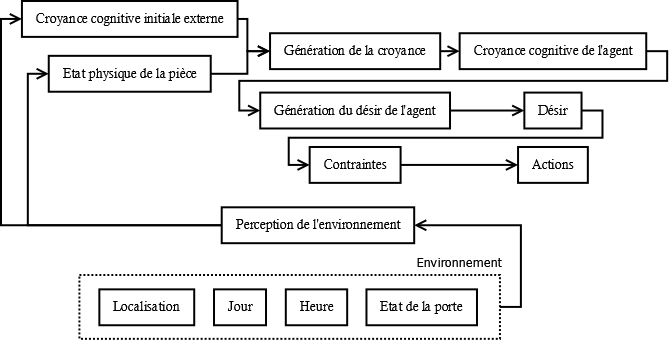
\includegraphics[scale=0.4]{Images/diagrammes_SMA/BRAHMS}
\caption{Diagramme représentant les éléments de la simulation sous BRHAMS pour la gestion de l'ouverture des portes}
\label{fig:Diagramme_BRAHMS}
\end{figure}

Malgré ce processus lourd propre à BRAHMS, Gaaloul et al. \cite{Gaaloul-12} l'ont couplé avec le logiciel COMFIE, afin de montrer l'intérêt de l'architecture à base de composant. Cette co-simulation entre COMFIE et BRAHMS est orchestrée par SIMULINK et apporte satisfaction dans les scénarios générés par BRAHMS, mais pas en terme de synchronisation et de temps de calculs. En effet, pour une simulation de 20 heures d'un bâtiment de deux zones, la durée de simulation est d'environ 20 minutes, soit plusieurs jours pour une simulation d'une année complète. 

\subsection{Repast}

Repast (\textit{REcursive Porous Agent Simulation Toolkit}) est une plateforme de modélisation et simulation avancée, gratuite et libre à base d'agents initialement développé à l'\textit{University of Chicago}. Il existe deux éditions, \textit{Repast Simphony} développé en Java, interactif et relativement facile à utiliser et \textit{Repast HPC (High-Performance Computing)} développé en C++ pour les experts qui utilisent des super-ordinateurs. Repast peut être codé sous plusieurs langages et peut intégrer des fonctions adaptatives, tels que des algorithmes génétiques, également appelés arbres de décision.

%Lacroix et al. \cite{Lacroix-12} a présenté ses travaux sur le contrôle des systèmes thermiques dans les bâtiments par gestion multi-agents. Ce projet a pour objectif d'optimiser la gestion de l'énergie en considérant l'impact économique  du prix de l'énergie. En plus de gérer la demande d'énergie, la gestion multi-agent au travers de Repast permet d'intégrer les sources d'énergies alternatives. L'architecture se base sur quatre types d'agents: des consommateurs, des producteurs, des distributeurs et des agents environnementaux. Le bâtiment est ici décrit comme un système multi-agent qui gère automatiquement les systèmes de contrôle thermique: chauffage, ventilation, air conditionné, production d'eau chaude sanitaire. Les résultats de cette étude montrent qu'un surcout de 2,5 \% entraine 35 \% de confort thermique supplémentaire.

Alfakara et Croxford \cite{Alfakara-14} utilisent Repast Simphony pour modéliser le comportement des occupants en confort estival dans les logements. Le modèle permet aux agents virtuels de Repast d'agir sur l'ouverture des fenêtres et sur l'activation de l'air conditionné. La modélisation des occupants se base sur la création d'agents: avec des propriétés individuelles (âge, style de vie, tolérance à la température, ...), autonomes et pouvant interagir entre eux. Le développement de ce modèle sous Repast permet par la suite d'étudier l'impact du comportement des occupants sur les consommations de climatisation. En effet, le SMA est couplé dynamiquement à un logiciel de simulation thermique, EDSL, qui traite le bâtiment et son environnement. Un objectif de cette étude est alors de comparer comment la manière de ce comporter vis à vis de la gestion des surchauffes modifie les consommations énergétiques. L'arbre de décision en Figure \ref{fig:Diagramme_Repast} montre le fonctionnement de Repast pour gérer les ouvertures de fenêtres et les actions sur la climatisation. Le processus décisionnel se présente alors comme un algorithme linéaire assez simple dans cet exemple, mais il peut être complexifié sans contrainte majeure. En amont de ce processus il est nécessaire de générer les agents et leurs propriétés intrinsèques.

\begin{figure}[H]
\centering
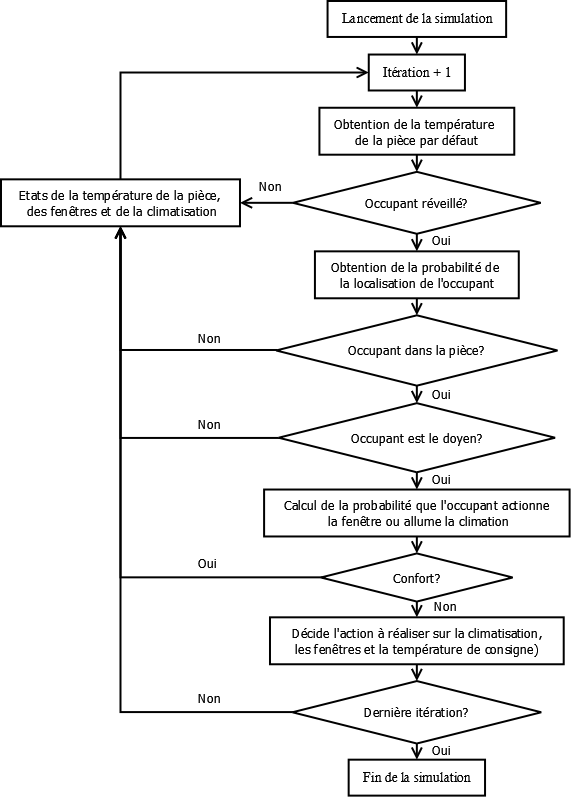
\includegraphics[scale=0.4]{Images/diagrammes_SMA/Repast}
\caption{Digramme décisionnel représentant les éléments de la simulation sous Repast pour la modélisation du confort estival}
\label{fig:Diagramme_Repast}
\end{figure}

\subsection{NetLogo}

NetLogo est une plateforme open-source SMA de modélisation de phénomènes collectifs. La plateforme est bien adaptée à la modélisation de systèmes complexes composés de centaines d'agents agissants en parallèle. La plateforme offre la possibilité de créer ses propres modèles constitués de trois types d'agents: les "\textit{turtles}" qui se déplacent dans leur environnement, les "\textit{patchs}" qui sont une portion statique de l'espace et les "\textit{observers}" qui organisent et donnent des instructions aux autres agents. NetLogo permet des modélisations des sciences sociales et naturelles de manière relativement simple.

Andrews et al. \cite{Andrews-11} ont utilisé NetLogo pour tester comment les bâtiments réagissent en fonction du comportements des occupants. Le comportement a été illustré sur l'application du confort des agents à la lumière et à son intensité. La modélisation du comportement des usagers sur la plateforme NetLogo doit pouvoir à terme être intégrée à une maquette numérique de type BIM. En effet, les limites du BIM peuvent être repoussées assez loin et une intégration des activités des occupants est à prévoir. Dans ces travaux, le lien est réalisé entre l'approche bien connue du BDI (\textit{Belief - Desire - Intension}) qui considère les croyances, les désires et les intentions des occupants et l'approche TPB (\textit{Theory of Planned Behaviour}) qui se base sur un modèle normalisé du comportement humain. L'objectif de ce couplage est alors de rendre la modélisation du comportement des occupants encore plus rationnelle que ce qui a l'habitude de se faire. La Figure \ref{fig:Diagramme_NetLogo} présente le processus décisionnel général correspondant qui mène à un comportement ou une action en utilisant la plateforme NetLogo. La modélisation dite de type \textit{BDI} est mise en évidence dans la première partie de l'algorithme puis la \textit{TPB} dans la deuxième, cela afin d'en définir l'état environnemental suivant.

\begin{figure}[H]
\centering
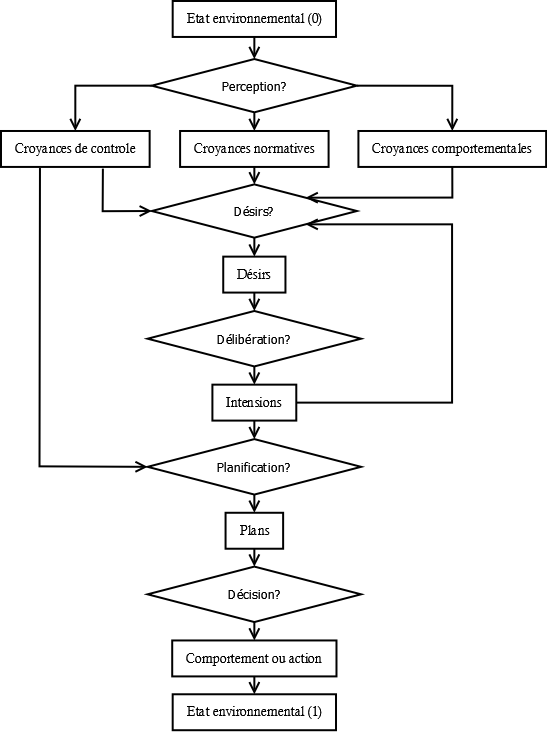
\includegraphics[scale=0.4]{Images/diagrammes_SMA/NetLogo}
\caption{Diagramme décisionnel représentant les éléments de la simulation sous NetLogo avec la combinaison \textit{BDI} et \textit{TPB}}
\label{fig:Diagramme_NetLogo}
\end{figure}

\subsection{OASys}

Cette sous-section est présentée différemment des autres puisque la plateforme OASys (\textit{Occupants’ Actions System}) fait partie de la deuxième catégorie de plateforme présenté dans ce chapitre. En effet, le développement par l'Université de Toulouse d'OASys a été codé sous JAVA pour ensuite être couplé à TRNSYS via C++. La modélisation du comportement des occupants n'utilise alors pas de plateforme pré-existante comme les travaux d'Andrews et al. \cite{Andrews-11}, d'Alfakara et Croxford \cite{Alfakara-14} ou encore de Tijani \cite{Tijani-14}.

Le cœur de la modélisation de Bonte \cite{Bonte-14} est basé sur le confort des occupants via un algorithme d'intelligence artificielle. Le modèle permet alors de prendre en compte les préférences interindividuelles et la simulation des actions des occupants en fonction de leurs sensations thermiques ou visuelles. L'unité de recherche couple par la suite la plateforme OASys avec le logiciel de Simulation Thermique Dynamique TRNSYS pour étudier l'influence du comportement des occupants sur la performance énergétique des bâtiments. La Figure \ref{fig:Diagramme_OASys} représente les éléments modélisés de la simulation sous OASys. Cela permet de bien visualiser que la modélisation de la part humaine est réalisée en deux étapes. Premièrement l'état physiologique est évalué par des modèles sur la sensation thermique et visuelle fins, et ensuite une réaction comportementale associée à une action est transmise à l'outil de STD pour en modifier l'environnement intérieur.

\begin{figure}[H]
\centering
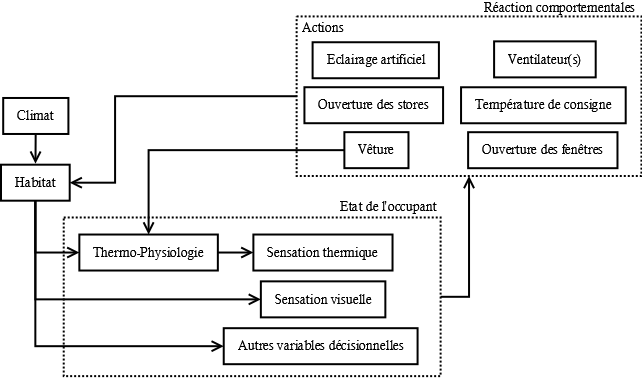
\includegraphics[scale=0.4]{Images/diagrammes_SMA/OASys}
\caption{Diagramme représentant les éléments de la simulation sous OASys avec la mise en avant de l'importance du confort}
\label{fig:Diagramme_OASys}
\end{figure}

\subsection{MASS}

Comme OASys, MASS (\textit{Multi-Agents Stochastic Simulation}) est une plateforme développée sans l'utilisation de plateforme SMA générale, mais développée sous C++ sur-mesure à la modélisation des individus dans les bâtiments. Ainsi, le développement de la plateforme et son utilisation sont réalisés au sein de la même unité de recherche.

MASS est développé par Robinson et son équipe et a pour objectif de réduire le \textit{performance gap} en mieux modélisant le caractère imprévisible des occupants. Cette plateforme développée par l'Université de Nottingham prend en compte les actions des occupants et leur nature imprévisible en couplant une modélisation stochastique avec une modélisation à base de systèmes multi-agents afin de servir le logiciel de simulation thermique EnergyPlus. Chapman et al. \cite{Chapman-14} précisent que la description de la structure (de la génération de ménages aux différents paramètres attribués à la simulation) ont une vraie utilité pour pouvoir étudier un large panel d'études de cas (résidentiel ou non résidentiel) sous différents climats. Le développement de MASS, sous C++, a été réalisé par l'utilisation de sous-modèles (activités, gains internes, ombrage, interactions entre les agents) qui sont testés par études de sensibilité pour sélectionner les plus influents et pour s'assurer que le modèle du comportement n'est pas trop lourd. La plateforme devant être lancée en 2015, il restait fin 2014, certains travaux à réaliser comme une meilleure adaptation pour le confort, l'ajout de nouveaux types de comportements, l'intégration de la modélisation de l'électricité spécifique ou encore des interactions entre les agents. Des modèles UML (\textit{Unified Modeling Language}) vont également être créés pour décrire comment les interactions fonctionnent et comment sont implémentées les règles pragmatiques dans la plateforme à base d'agents. Les règles qui auront un impact significatif sur la performance des bâtiments vont donc permettre de savoir où les futurs efforts doivent être faits pour créer de nouveaux modèles valides. La Figure \ref{fig:Diagramme_MASS} présente le diagramme décisionnel général du modèle MASS. Celui-ci nous permet de mieux visualiser les différents composants de la plateforme, c'est à dire le pré-processus, les agents et les actions associées. L'association de la plateforme au logiciel EnergyPlus permet alors une modélisation plus complète des bâtiments.

\begin{figure}[H]
\centering
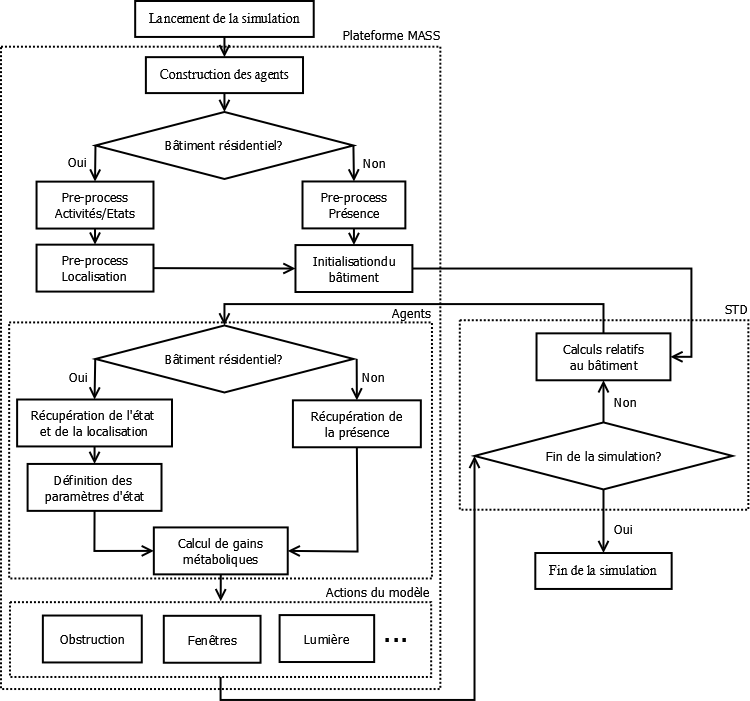
\includegraphics[scale=0.4]{Images/diagrammes_SMA/MASS}
\caption{Diagramme décisionnel représentant les éléments de la simulation sous MASS et la liaison avec EnergyPlus}
\label{fig:Diagramme_MASS}
\end{figure}

\subsection{Composant W de TRNSYS}

Bien que dans ce chapitre sur le choix de plateforme, ce paragraphe est justifié dans le sens où le composant W proposé par le logiciel TRNSYS permet de développer des composants dans un langage simple et spécialement conçu pour la simulation dynamique. Le potentiel de ce composant a été étudié pour savoir s'il pouvait recréer toutes les fonctionnalités de MASS ou d'autres modèles de comportement pour une application en bureaux d'études.

Ce composant à vil prix de 195 \euro{} \footnote{http://boutique.cstb.fr/Product/langage-w} permet une extension illimitée par bloc de TRNSYS sur une interface conviviale et sous un développement de haut niveau (langage W), c'est à dire éloigné de la machine et sans gestion de mémoire. L'utilisation du composant W simplifie le code lourd généré par l'utilisation des FMU, DLL, XML et autres scripts Python(cf chap suivant) qui servent à la co-simulation entre le logiciel de STD et la plateforme de modélisation des comportements.

En revanche, et bien que l'utilisation du composant W de TRNSYS simplifie la gestion par son approche modulaire, ce langage est bridé car il ne permet pas l'intégration de bibliothèque externe et empêche la modélisation de certains aspects comme le bouclage général de la simulation. Aussi, cela implique de re-coder en W des modèles qui existent ce qui demande un investissement en temps considérable. Enfin, le pré-processus de la simulation sous W est très difficilement géré gracieusement car il nécessite l'utilisation d'un logiciel externe, tout comme des fichiers XML avec MASS par exemple: cela n'aboutissant donc pas à la simplification d'utilisation par rapport à une co-simulation. 

Cette sous-section apparait donc ici comme un bonus aux plateformes de modélisation du comportement des occupants existants puisque seul le composant W ne permet pas le développement d'une plateforme. Il découle donc d'une réflexion sur son pouvoir de remplacer les plateformes traditionnelles utilisées en co-simulation avec les logiciels thermiques dynamique. Co-simulation qui semble en l'état ingérable pour des industriels de type bureaux d'études.

\section{Synthèse}

L'étude de la modélisation du comportement des usagers des bâtiments nous a amener à constater que par le passé plusieurs approches avaient été réalisées. Des plus simples comme les modèles basés sur des valeurs moyennes ou des scénarios déterministes au plus modernes comme les modèles à base d'agents, tous ont leurs avantages et inconvénients. Un des objectifs de la thèse étant de faire gagner aux outils de Simulation Thermique Dynamique de la fiabilité par une prise en compte plus réaliste des comportements humains, il nous a semblé logique de nous orienter vers une approche suffisamment détaillée et proche de la réalité. Le choix du type de modèle s'est alors porté d'une part vers les Systèmes Multi-Agents pour modéliser la singularité des individus mais également d'autre part à une modélisation stochastique pour modéliser la part d'aléatoire du comportement.

Les outils permettant de modéliser les comportements à base de SMA sont synthétisés dans le tableau \ref{tab:syntheseSMA}. Il permet  de révéler la diversité des approches et la maturation des projets.

\begin{table}[h]
\begin{center}
\begin{tabular}{{|p{3cm}||p{2.5cm}|p{2.5cm}|p{3.5cm}|p{3.5cm}|}}
\hline Plateforme - [Référence] & Reprise d'une plateforme générale & Outils STD & Potentiel de finesse de la modélisation & Fonctionnalité en BE \\
\hline
\hline BRAHMS - \newline Tijani et al. \cite{Tijani-14} & Oui & Pas encore couplé & Très fin - basé sur les sciences cognitives & Quasi impossible: demande un énorme travail \\
\hline Repast - \newline Alfakara et al. \cite{Alfakara-14} & Oui & EDSL 2012 & Moyen - basé sur le bon sens du modélisateur & Non - Application spécifique au confort estival \\
\hline NetLogo - \newline Andrews et al. \cite{Andrews-11} & Oui & MATLAB & Fin - basé sur les théories \textit{BDI} et \textit{TPB} & Possible - Modèle comportemental à simplifier \\
\hline OASys - \newline Bonte et al. \cite{Bonte-14} & Non & TRNSYS & Fin  - basé sur le confort thermique et visuel & Modèle comportemental à simplifier \\
\hline MASS - \newline Chapman et al. \cite{Chapman-14} & Non & EnergyPlus & Moyen - basé sur des comportements réactifs & Assez difficilement à l'heure actuelle \\
\hline Composant W & Non & TRNSYS & Grossier - L'impossibilité d'insérer des bibliothèques bride le développement & Totale \\
\hline
\end{tabular}
\caption{Synthèse des modèles à base d'agents servant à créer un lien avec un outil STD}
\label{tab:syntheseSMA}
\end{center}
\end{table}

Suite à la revue des travaux réalisés modélisant les occupants et leurs comportements par des simulations multi-agents, trois choix se sont opposés. Le premier consistait à utiliser une plateforme multi-applications pour ensuite développer les modèles comportementaux. Cette première option avait l'avantage de pouvoir développer des agents cognitifs évolués en exploitant pleinement le potentiel des SMA et de l'intelligence artificielle mais le développement fin qu'implique ces plateformes allait à l'encontre des objectifs initiaux de proposer une modélisation globale et exploitable des comportements. Le second choix était d'intégrer en cours de développement une unité de recherche. L'\textit{annex 66} a permis de rencontrer Robinson de l'Université de Nottingham, précurseur dans le domaine, avec qui une synergie a été évoquée. Cette option avait l'avantage de poursuivre et de récupérer des travaux en cours mais impliquait une mise à niveau importante principalement en terme de logique informatique d'autant plus délicate que le laboratoire partenaire était géographiquement peu accessible. La troisième option était de reprendre le fond du travail de Nottingham sous l'éditeur de composant dynamique de TRNSYS mais dans simplifier la forme. L'avantage principal à cette option était de pouvoir proposer, à terme, des composants plus modulaires et accessibles pour un bureau d'étude technique que du code primitif C++ et des fichiers xml. L'inconvénient de cette option était le manque de puissance nécessaire pour obtenir une plateforme complète, ce choix  

Le choix final c'est porté sur la collaboration avec l'université de Nottingham, la plateforme MASS (\textit{Multi-Agents Stochastic System}) et son application sont donc l'objet de la partie suivante.

